\documentclass[12pt]{article}

\usepackage{amsmath}
\usepackage{amssymb}
\usepackage{geometry}
\usepackage{enumitem}
\usepackage{tikz}
\usetikzlibrary{
    arrows.meta,
    calc,
    angles,
    quotes,
    decorations.pathmorphing
}
\usepackage[american]{circuitikz}


\geometry{margin=1in}

\begin{document}

\begin{enumerate}[leftmargin=*]

\item One mole of an ideal gas is taken quasi-statically from $(P_0,V_0)$ to $(2P_0,2V_0)$ along a straight line in the $P$–$V$ plane such that pressure varies linearly with volume, and during the process the temperature first decreases slightly before rising to its final value. Using ideal gas law and eliminating temperature, the work must be computed by integrating the exact linear relation rather than using average pressure. The internal energy change must also be compared with the net heat supplied to ensure consistency. Determine the total work done by the gas in terms of $P_0V_0$.

A) $\dfrac{3}{2}P_0V_0$

B) $2P_0V_0$

C) $\dfrac{5}{2}P_0V_0$

D) $3P_0V_0$

\item An ideal gas undergoes a cyclic process consisting of isothermal expansion at temperature $T_{\max}$, followed by an adiabatic compression back to the initial state at $T_{\min}$, with $T_{\max}=2T_{\min}$. The expansion ratio is such that the adiabatic exactly restores the original volume and pressure, and the specific heat ratio is $\gamma$. Using coupled isothermal work and adiabatic relation $TV^{\gamma-1}=\text{constant}$, determine the efficiency of this engine after eliminating intermediate volumes.

% Diagram for Question 2
\begin{center}
\begin{tikzpicture}[scale=1.1]

% Axes
\draw[->] (0,0) -- (6,0) node[right] {$V$};
\draw[->] (0,0) -- (0,5) node[above] {$P$};

% State A
\coordinate (A) at (1.2,3.4);

% Isothermal constant
\pgfmathsetmacro{\K}{1.2*3.4}

% State B on isothermal
\coordinate (B) at (4.5,{\K/4.5});

% Isothermal A→B
\draw[thick,domain=1.2:4.5,smooth,variable=\x]
plot ({\x},{\K/(\x)});

% Adiabatic B→A using PV^gamma = const
\pgfmathsetmacro{\gamma}{1.4}
\pgfmathsetmacro{\C}{3.4*(1.2^\gamma)}

\draw[thick,domain=4.5:1.2,smooth,variable=\x]
plot ({\x},{\C/(\x^\gamma)});

% Points
\fill (A) circle (2pt);
\fill (B) circle (2pt);

\node[left] at (A) {$A$};
\node[right] at (B) {$B$};

\node[right] at (4.6,1.5) {\small Isothermal};
\node at (2.2,3.2) {Adiabatic};

\end{tikzpicture}
\end{center}

A) $1-2^{-(\gamma-1)/\gamma}$

B) $1-\dfrac{1}{2}$

C) $1-2^{-(\gamma-1)}$

D) $1-\dfrac{1}{2^{1/\gamma}}$

\item A parallel-plate capacitor of plate area $A$ and separation $d$ is half-filled along the area (not thickness) by a dielectric of constant $k$, the interface being parallel to the electric field. Fringing is neglected, but the charge redistributes so that potential difference across both regions remains identical. Using field continuity and parallel combination reasoning, determine the equivalent capacitance in exact symbolic form.

% Diagram for Question 3

\begin{center}
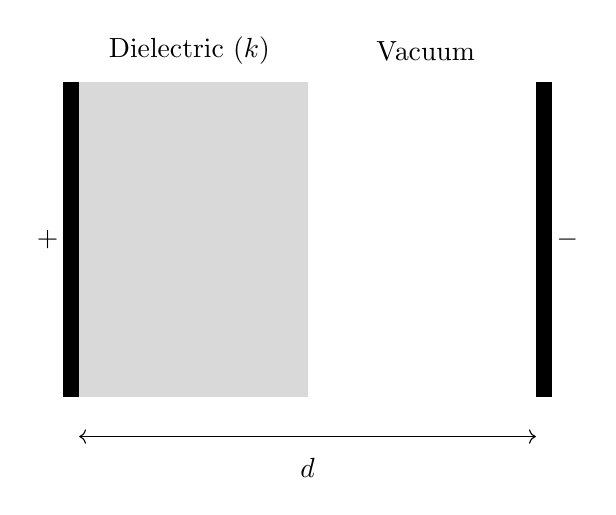
\begin{tikzpicture}[scale=1]

% Plates
\fill[black] (-0.1,0) rectangle (0.1,4);
\fill[black] (5.9,0) rectangle (6.1,4);

% Dielectric region (half area)
\fill[gray!30] (0.1,0) -- (3,0) -- (3,4) -- (0.1,4) -- cycle;

% Labels
\node at (-0.3,2) {$+$};
\node at (6.3,2) {$-$};
\node at (1.5,4.4) {Dielectric ($k$)};
\node at (4.5,4.4) {Vacuum};

% Separation
\draw[<->] (0.1,-0.5) -- (5.9,-0.5);
\node at (3,-0.9) {$d$};

\end{tikzpicture}
\end{center}

A) $\dfrac{\epsilon_0A}{d}\dfrac{k+1}{2}$

B) $\dfrac{\epsilon_0A}{d}\dfrac{2k}{k+1}$

C) $\dfrac{\epsilon_0A}{d}(k+1)$

D) $\dfrac{\epsilon_0A}{d}\sqrt{k}$

\item A dipole consists of charges $+q$ and $-q$ separated by distance $2a$. The electric field is to be evaluated at a point on the perpendicular bisector at a distance $a$ from the midpoint. Without using far-field approximation, resolve vector components exactly and simplify by symmetry cancellation, ensuring no premature dipole approximation is applied. Determine the magnitude of the field.

% Diagram for Question 4
\begin{center}
\begin{tikzpicture}[scale=1]

% Charges
\fill (-2,0) circle (3pt);
\fill (2,0) circle (3pt);

\node[below] at (-2,0) {$+q$};
\node[below] at (2,0) {$-q$};

% Line joining charges
\draw (-2,0) -- (2,0);

% Midpoint
\filldraw[black] (0,0) circle (1.5pt);

% Perpendicular bisector
\draw[dashed] (0,-3) -- (0,3);

% Field point at distance a
\fill (0,2) circle (3pt);
\node[right] at (0,2) {$P$};

% Distance marking
\draw[<->] (0,0) -- (0,2);
\node[right] at (0,1) {$a$};

\node[below] at (0,0) {Midpoint};

\end{tikzpicture}

\end{center}
A) $\dfrac{kq}{2\sqrt2\,a^2}$

B) $\dfrac{kq}{\sqrt2\,a^2}$

C) $\dfrac{2kq}{\sqrt2\,a^2}$

D) $\dfrac{kq}{a^2}$

\item A capacitor of capacitance $C$ initially charged to $V_0$ discharges through a resistor $R$. The instantaneous power dissipated in the resistor depends on both the decaying voltage and current simultaneously. By differentiating the exact expression $P(t)=\dfrac{V_0^2}{R}e^{-2t/RC}$ and carefully checking extrema conditions, determine the time at which power falls to half of its initial maximum value.

A) $\dfrac{RC}{2}\ln2$

B) $RC\ln2$

C) $\dfrac{RC}{4}\ln2$

D) $\dfrac{RC}{2}$

\item In a Wheatstone bridge initially balanced with all arms $R$, one arm is changed to $R+\Delta R$ with $\Delta R \ll R$. The battery emf is $E$ and galvanometer resistance is negligible. Using first-order perturbation and eliminating node potentials through simultaneous equations, determine the galvanometer current magnitude to first order in $\Delta R/R$.

% Diagram for Question 6

\begin{center}
\begin{circuitikz}[american]

% Nodes
\coordinate (Top) at (2,4);
\coordinate (Left) at (0,2);
\coordinate (Right) at (4,2);
\coordinate (Bottom) at (2,0);

% Resistors
\draw (Left) to[R,l={$R$}] (Top);
\draw (Top) to[R,l={$R$}] (Right);
\draw (Right) to[R,l={$R+\Delta R$}] (Bottom);
\draw (Bottom) to[R,l={$R$}] (Left);

% Galvanometer
\draw (Top) to[ammeter,l={$G$}] (Bottom);

% Battery
\draw (Left) -- ++(0,-1) coordinate (Lbot);
\draw (Right) -- ++(0,-1) coordinate (Rbot);
\draw (Lbot) to[battery,l={$E$}] (Rbot);
\draw (Lbot) -- (Left);
\draw (Rbot) -- (Right);

\end{circuitikz}
\end{center}

A) $\dfrac{E}{4R}\dfrac{\Delta R}{R}$

B) $\dfrac{E}{2R}\dfrac{\Delta R}{R}$

C) $\dfrac{E}{8R}\dfrac{\Delta R}{R}$

D) $\dfrac{E}{R}\dfrac{\Delta R}{R}$

\item For Maxwell speed distribution at temperature $T$, the most probable speed is $v_p$. Using the distribution’s skewness and normalization properties (without performing full integration), determine the fraction of molecules having speed greater than $v_p$, considering that the distribution is asymmetric about $v_p$.

A) Greater than $\dfrac{1}{2}$

B) Exactly $\dfrac{1}{2}$

C) Less than $\dfrac{1}{2}$ but finite

D) Infinitesimal

\item An isolated capacitor of capacitance $C$ is charged and then a dielectric of constant $k$ is inserted fully between plates without touching them. Charge remains constant while electric field and potential redistribute. Using energy density and field scaling arguments, determine the fractional change in stored energy.

A) Decreases by factor $1/k$

B) Increases by factor $k$

C) Remains same

D) Decreases by factor $1/k^2$

\item A battery of emf $E$ and internal resistance $r$ supplies power to load $R$. If load resistance is slightly perturbed from the maximum power condition as $R=r(1+\epsilon)$ with $|\epsilon|\ll1$, determine the fractional decrease in delivered power to first order in $\epsilon$.

A) $\epsilon^2$

B) $\epsilon$

C) $\dfrac{\epsilon}{2}$

D) Zero (to first order)

\item A uniformly charged ring of radius $R$ produces an axial electric field $E(x)=\dfrac{kQx}{(R^2+x^2)^{3/2}}$. By differentiating with respect to $x$ and solving the extremum condition exactly, determine the axial position where field magnitude is maximum.

% Diagram for Question 10

\begin{center}
\begin{tikzpicture}[scale=1]

% Ring
\draw[thick] (0,0) circle (2);

% Axis
\draw[dashed] (0,-4) -- (0,4);
\fill (0,3) circle (3pt);
\node[right] at (0,3) {$P(x)$};

% Radius label
\draw (0,0) -- (2,0);
\node[above] at (1,0.2) {$R$};

% Center
\fill (0,0) circle (2pt);
\node[below left] at (0,0) {\small O};

\end{tikzpicture}
\end{center}

A) $x=\dfrac{R}{\sqrt2}$

B) $x=R$

C) $x=\dfrac{R}{2}$

D) $x=\sqrt2\,R$

\item An ideal gas undergoes a free expansion into vacuum inside an insulated container doubling its volume. Using entropy expression for ideal gas and eliminating temperature change via energy conservation, determine the entropy change per mole.

A) $R\ln2$

B) Zero

C) $-R\ln2$

D) $\dfrac{R}{2}\ln2$

\item For an electrostatic field $\vec E=-\nabla V$, consider a small displacement $d\vec r$ along an equipotential surface where $dV=0$. Using scalar product structure, determine which mathematical property enforces perpendicularity between $\vec E$ and equipotential surface.

A) $\vec E\cdot d\vec r=0$

B) $\vec E\times d\vec r=0$

C) $\nabla\cdot\vec E=0$

D) $\nabla\times\vec E=0$

\item A linear dielectric slab inserted in uniform field develops polarization $\vec P=\epsilon_0\chi_e\vec E_{\text{net}}$. Using superposition of applied and induced fields and eliminating bound surface charge density, determine the ratio of net electric field to applied external field.

A) $\dfrac{1}{1+\chi_e}$

B) $1+\chi_e$

C) $\chi_e$

D) $\dfrac{\chi_e}{1+\chi_e}$

\item In a conductor carrying steady current, electrons have thermal speed $v_{th}$ and drift velocity $v_d$. Using random walk arguments and relaxation time $\tau$, determine the ratio $v_d/v_{th}$ in terms of electric field $E$, charge $e$, mass $m$, and thermal speed.

A) $\dfrac{eE\tau}{mv_{th}}$

B) $\dfrac{eE}{m}$

C) $\dfrac{v_{th}}{eE\tau}$

D) Independent of $v_{th}$

\item A Carnot engine operates between reservoirs at $T_h$ and $T_c$. If both temperatures are increased by the same small fraction $\delta$ while maintaining $T_h-T_c$ constant, determine the first-order fractional change in efficiency.

A) Decreases

B) Increases

C) Zero to first order

D) Doubles

\end{enumerate}

\end{document}